\documentclass[pdf]{beamer}
\mode<presentation>{}
\usepackage{minted}
\usepackage{tikz,tikz-3dplot}
\usepackage{pgffor} %% gives looping with \foreach
\usepackage[absolute,overlay]{textpos}
\usepackage{lmodern} %% scalable latin characters
\usetikzlibrary{arrows,shapes,backgrounds}
\usepackage{multirow}
\usepackage{listings} %% another package for code related stuff
%\usepackage[fleqn]{amsmath}

%% stuff for minted
\definecolor{mintedBg}{rgb}{0.95, 0.95, 0.95}
\definecolor{blockBg}{rgb}{0.6, 0.6, 0.95}
\definecolor{rnaColor}{rgb}{0, 0.6, 0}
\definecolor{cdsColor}{rgb}{0, 0.4, 0.4}
\definecolor{rnaPol}{rgb}{0.8,0,0.8}
\definecolor{ribosomeCol}{rgb}{0.5,0.5,0.1}
\definecolor{protColor}{rgb}{0.6,0,0.6}
%% colours for nucleotides:
\definecolor{dACol}{rgb}{0.5, 0.5, 0}
\definecolor{dCCol}{rgb}{0.8, 0, 0}
\definecolor{dGCol}{rgb}{0, 0.8, 0}
\definecolor{dTCol}{rgb}{0, 0, 0.8}

\definecolor{navy}{rgb}{0, 0, 0.6}
\definecolor{pur}{rgb}{0, 0, 0.6}
\definecolor{pyr}{rgb}{0.6, 0, 0.2}

\definecolor{purple1}{rgb}{1.0, 0, 0.6}
\definecolor{purple2}{rgb}{0.8, 0, 0.8}
\definecolor{purple3}{rgb}{0.6, 0, 1.0}
%% define styles for different codes
\newminted{cpp}{linenos, bgcolor=blockBg, fontsize=\footnotesize}
%% then use \begin{cppcode}
\newminted{c}{linenos, bgcolor=mintedBg, fontsize=\footnotesize}
\newminted{perl}{linenos, bgcolor=mintedBg, fontsize=\footnotesize}
\newminted{r}{linenos, bgcolor=mintedBg, fontsize=\tiny}

%% a command to define a subheading
\newcommand\subHeading[1]{
  \par\bigskip {\Large\bfseries#1}\par\smallskip
}

%% I detest indentation in footnotes etc, so try this:
\makeatletter
\renewcommand\@makefntext[1]{\noindent\makebox[0em][r]{\@makefnmark}\tiny#1}
\makeatother
%% the makeatletter and makeatother are required to allow me to
%% to change the macro beginning with an @. (though when I call it
%% I don't use the @ ... 

\setlength\parskip{0.5em}
\setlength\parindent{0ex}

%% to have footnotes without references. This from tex.stackexchange.com
\newcommand\blfootnote[1]{%
  \begingroup  %% this makes it a local redefinition
  \renewcommand\thefootnote{}\footnote{#1}%
  \addtocounter{footnote}{-1}  % this adjusts the footnote counter
  \endgroup
}


%% to draw a pair of genes..
\newcommand{\genePair}[3][]{
        \draw [-,#1] (#2-1,#3) -- (#2+1,#3);
        \draw [-,line width=2, purple1] (#2-0.5,#3) -- (#2+0.5,#3);
        \draw [-,#1] (#2-1,#3-0.5) -- (#2+1,#3-0.5);
        \draw [-,line width=2, purple3] (#2-0.5,#3-0.5) -- (#2+0.5,#3-0.5);  
}

\title{Looking at big Data sets}
\subtitle{visualising data}
\author{Martin Jakt}

\begin{document}

\begin{frame}
\titlepage
\end{frame}

\begin{frame}{What kind of experiments}
  \begin{itemize}
    \small
  \item DNA sequence
    \begin{itemize}
      \footnotesize
    \item DNA assembly
    \item variant detection \& analysis (evolution \& cancer)
    \item genome comparisons (evolution)
    \end{itemize}
  \item gene expression
    \begin{itemize}
      \footnotesize
    \item Microarrays
    \item RNA-seq
    \end{itemize}
  \item protein DNA interaction
    \begin{itemize}
      \footnotesize
    \item chromatin Immuno-Precipitation (ChIP) - chip
    \item ChiP-seq
    \end{itemize}
  \item DNA methylation
  \item protein RNA interaction
  \item protein protein interactions (eg. high throughput yeast two-hybrid)
  \item Chromatin configuration (Hi-C, identifies long-range genomic interactions)
  \item ...
  \end{itemize}
  
  \small limited by technology
\end{frame}

\begin{frame}{Data types}
  Several steps in the processing pipeline. Starting data is usually image data
  which gets converted to signal intensities or sequences which are in turn
  converted to some sort signal.

  Processed data:
  \begin{itemize}
  \item Gene based:\\
    one value / gene / sample
  \item Location based:\\
    one value / location / sample
  \item Interaction based:\\
    one value / unit / unit (/ sample)\\
    unit = protein or location 
  \end{itemize}
\end{frame}

\begin{frame}{RNA expression: microarray}
  \begin{enumerate}
  \item mRNA $\Rightarrow$ cDNA $\Rightarrow$ labelled cRNA
  \item applied to array with immobilised probe sequences:\\
    $\sim$1e6 probes.
  \item signal intensity $\Rightarrow \sim$ transcript abundance
  \end{enumerate}
\end{frame}

\begin{frame}{RNA expression: NGS}
NGS: next generation sequencing.

DNA sequence determined by extending immobilised DNA molecules one
or two bases at a time. Sequence determined by image analysis.

mRNA $\Rightarrow$ [fragmented] cDNA $\Rightarrow$ sequence data

number of reads mapping to a given transcript $\sim$ transcript abundance
\end{frame} 

\begin{frame}{Chromatin Immuno-Precipitation}
  commonly referred to as CHIP

  \begin{enumerate}
  \item chromatin fixed by crosslinking to proteins
  \item  fragmented (usually by sonication)
  \item  DNA fragments bound to specific protein or modification
    are enriched by immunoprecipitation with antibody
  \item Extent of enrichment determined by hybridisation to microarrays
    (ChIP-chip) or by high throughput sequencing (ChIP-seq)
  \end{enumerate}

  Enrichment indicates probability or strength of interactions
\end{frame}

\begin{frame}{the Data}
  \begin{figure}[ht]
    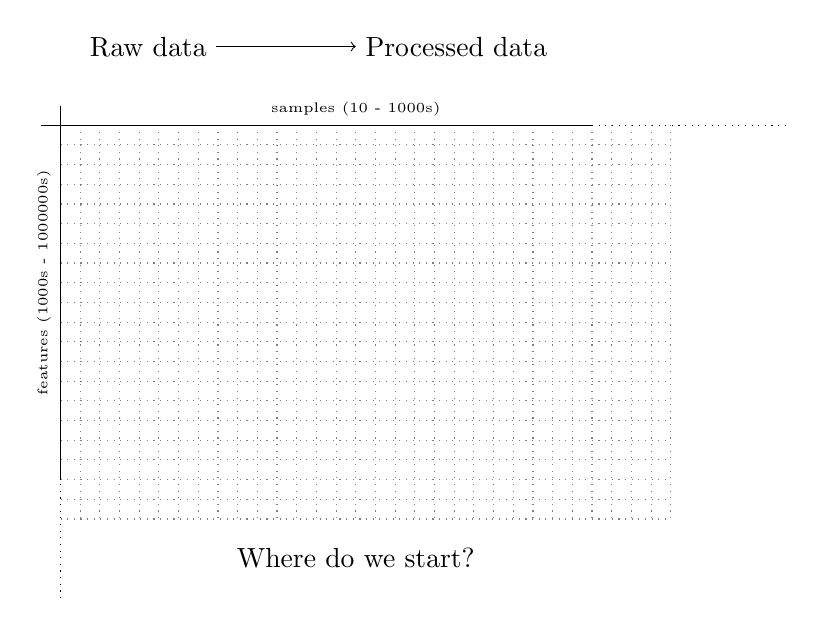
\begin{tikzpicture}[scale=0.5]
%      \draw [help lines, opacity=0] (0,0) grid (22,12);
%      \foreach \x in {1,2,...,19} \node [font=\small] at (\x,0) {\x};
%      \foreach \y in {1,2,...,12} \node [font=\small] at (20,\y) {\y};
      \node [right] (l1) at (1,12) {Raw data};
      \node [right] (l2) at (8,12) {Processed data};
      \draw [->] (l1) -- (l2);
      
      \draw [-, dotted] (0,10) -- (19,10);
      \draw [-] (0,10) -- (14,10);
      \draw [-, dotted] (0.5, 10.5) -- (0.5, -2);
      \draw [-] (0.5, 10.5) -- (0.5, 1);

      \foreach \x in {1, 1.5, ...,16} \draw [-,dotted, opacity=0.5] (\x,10) -- (\x,0);
      \foreach \y in {9.5, 9, ...,0} \draw [-,dotted, opacity=0.5] (0.5,\y) -- (16,\y);

      \node [above, rotate=90] at (0.5,6) {\tiny features (1000s - 1000000s)};
      \node [above] at (8,10) {\tiny samples (10 - 1000s)};

      \node [below] at (8,-0.5) {Where do we start?};
%      \draw [->] (5, 11) node (l1) [left] {Raw data} -- (10,11) node (l2) [right] {Processed data};
      
  \end{tikzpicture}
\end{figure}
\end{frame}

\begin{frame}{the metaData}
  about the experiment:
  \begin{figure}[ht]
    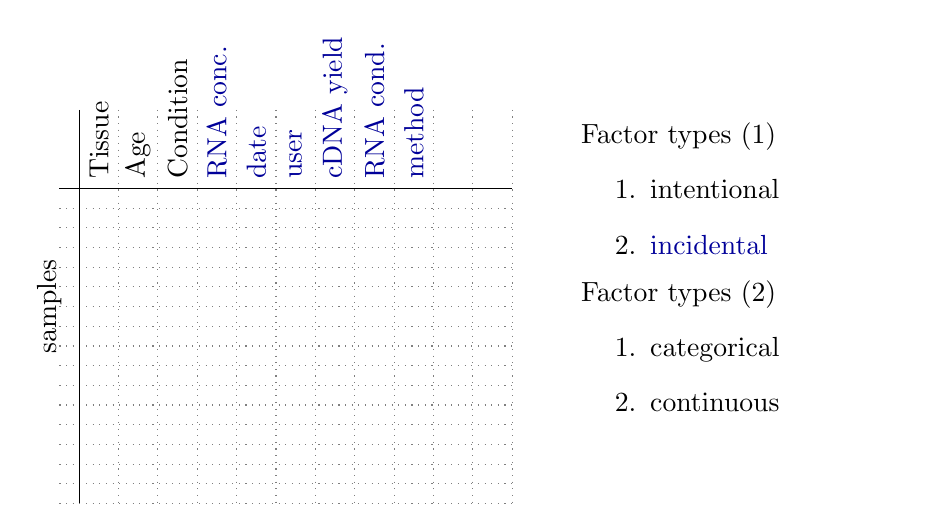
\begin{tikzpicture}[scale=0.5]
%      \draw [help lines, opacity=0.5] (0,0) grid (22,12);
%      \foreach \x in {1,2,...,19} \node [font=\small] at (\x,0) {\x};
%      \foreach \y in {1,2,...,12} \node [font=\small] at (20,\y) {\y};
      \node [right, rotate=90] at (1,8) {Tissue};
      \node [right, rotate=90] at (2,8) {Age};
      \node [right, rotate=90] at (3,8) {Condition};
      \node [right, rotate=90, navy] at (4,8) {RNA conc.};
      \node [right, rotate=90, navy] at (5,8) {date};
      \node [right, rotate=90, navy] at (6,8) {user};
      \node [right, rotate=90, navy] at (7,8) {cDNA yield};
      \node [right, rotate=90, navy] at (8,8) {RNA cond.};
      \node [right, rotate=90, navy] at (9,8) {method};
      
      \draw [-] (0,8) -- (11.5,8);
      \draw [-] (0.5,10) -- (0.5,0);
      \node [above, rotate=90] at (0.3,5) {samples};
      \foreach \x in {1.5, 2.5, ..., 11.5} \draw [-,dotted, opacity=0.5] (\x,10) -- (\x,0);
      \foreach \y in {7.5, 7, ..., 0} \draw [-,dotted, opacity=0.5] (0,\y) -- (11.5,\y);

      \node [right, align=left, text width=4cm] at (13,8) {
        Factor types (1)
        \begin{enumerate}
          \item intentional
          \item \textcolor{navy}{incidental}
        \end{enumerate}
        };
      \node [right, align=left, text width=4cm] at (13,4) {
        Factor types (2)
        \begin{enumerate}
          \item categorical
          \item continuous
        \end{enumerate}
        };
    \end{tikzpicture}
  \end{figure}
  normally more incidental than intentional factors...
\end{frame}

\begin{frame}{more metaData}
  features
  \begin{itemize}
  \item Transcripts
    \begin{itemize}
    \item gene id
    \item gene properties (location, function, molecular properties, ...)
    \item probe location / spliceform specificity
    \end{itemize}
  \item Locations \& proximity information
    \begin{itemize}
    \item transcripts (i.e. genes)
    \item gene features (eg. promoter, intron / exon boundaries, 
      CpG islands, other annotation).
    \end{itemize}
  \end{itemize}
  not strictly required for analysis, but needed for data-mining
  (identifying features that have some biological importance).
\end{frame}

\begin{frame}{the analysis}
  \begin{figure}[ht]
    \begin{tikzpicture}[scale=0.5]
%      \draw [help lines, opacity=0.5] (0,0) grid (22,12);
%      \foreach \x in {1,2,...,19} \node [font=\small] at (\x,0) {\x};
%      \foreach \y in {1,2,...,12} \node [font=\small] at (20,\y) {\y};
      \draw [-] (1,10) -- (5,10);
      \draw [-] (1.2,10.2) -- (1.2,6);
      \draw [-] (1,4) -- (5,4);
      \draw [-] (1.2,4.2) -- (1.2, 0);
      \draw [-] (11,9) -- (14,9);
      \draw [-] (11.2,9.2) -- (11.2, 2);

      \node [above, align=left] at (3,10) {Sample\\data};
      \node [above, align=left] at (3,4) {feature\\data};
      \node [above, align=left] at (12.5,9) {Data};
      
      \visible<2->{
        \node [align=center] (l1) at (7,6) {do\\something\\smart};
        \draw [->] (5,8) -- (l1);
        \draw [->] (5,2) -- (l1);
        \draw [->] (11,5) -- (l1);
      }
    \end{tikzpicture}
  \end{figure}
\end{frame}

\begin{frame}{a typical analysis pipeline}

  {\small
  \begin{enumerate}
  \item Work out what the samples are. (Usually means talk to
    the people doing the experiment; preferrably before the experiment).
  \item Do some general quality control. Normalise within samples if necessary.
  \item Look at overall patterns within the data. Look at how they correlate
    with the sample annotation (i.e. metadata).
  \item Go back to the experimentalists and get them to explain stuff that
    they didn't think you'd need to know and which complicate the analysis.
  \item Look at individual features to understand how the data varies.
  \item Extract interesting features (that correlate with sample factors)
  \item Potentially formulate some question and see if the data can support 
    this.\footnote{This is common, but a bad practice. Ideally the questions
      should be defined prior to the experiment. If statistical proof is required
      then the methods also need to be defined before looking at the data. We
      don't generally do this though.}
  \end{enumerate}
}
\end{frame}

\begin{frame}{Normalisation}

  {\small
  In the simplest form, normalisation is used as a loading control.
  eg.

  Sample A $\Rightarrow$ 100 ng labelled probe\\
  Sample B $\Rightarrow$ 20 ng labelled probe\\

  when transcript levels in sample A and B are measured on a microarray,
  transcripts from A will tend to have higher levels. We can correct for
  this by simply dividing by the overall signal from each sample.

  In more complex cases we can get changes in distributions that are not
  linear (interaction between sample and experimental limitations). \\
  There are a lots of ways to handle this. The most brutal one is:

  Quantiles normalisation: forces every sample to have the same distribution of
  signal strengths.

  RNA-seq data is usually implicitly normalised by sequence depth; but comparing
  RNA-seq data of different depth of sequencing is difficult.
}
\end{frame}

\begin{frame}{quantiles normalisation}

  \begin{enumerate}
  \item sort values from each sample
  \item calculate mean values for each rank
  \item assign mean values back by rank
  \end{enumerate}

  \begin{figure}[ht]
    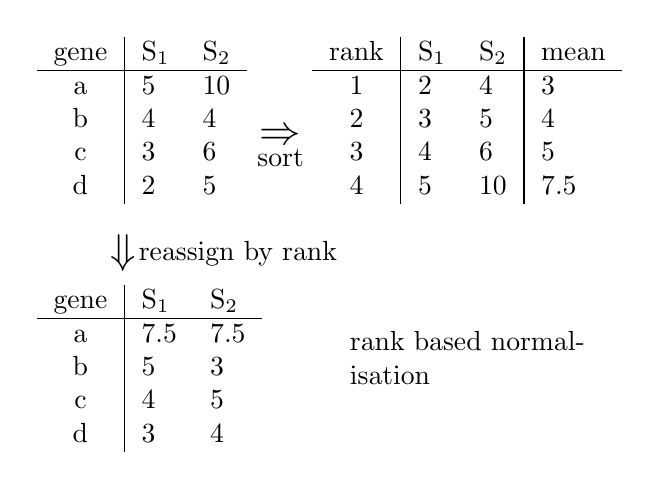
\begin{tikzpicture}[scale=0.35]
     %% \draw [help lines, opacity=0.5] (0,0) grid (22,10);
     %% \foreach \x in {1,2,...,19} \node [font=\small] at (\x,0) {\x};
     %% \foreach \y in {1,2,...,10} \node [font=\small] at (20,\y) {\y};
     
     \node [below right, align=left, text width=4cm] at (0,12) {
       \begin{tabular}{c|ll}
         gene & S$_1$ & S$_2$ \\
         \hline
         a & 5 & 10 \\
         b & 4 & 4 \\
         c & 3 & 6 \\
         d & 2 & 5 \\
       \end{tabular} };

     \visible<2->{
       \node [scale=1.5] at (9.2,8) {$\Rightarrow$};
       \node [below] at (9.2,7.9) {sort};
       \node [below right, align=left, text width=4cm] at (10,12) {
         \begin{tabular}{c|ll|l}
           rank & S$_1$ & S$_2$ & mean \\
           \hline
           1 & 2 & 4 &  3\\
           2 & 3 & 5 & 4 \\
           3 & 4 & 6 & 5\\
           4 & 5 & 10 & 7.5\\
       \end{tabular} };
     }
     \visible<3->{
       \node [scale=1.5] at (3.5,3.8) {$\Downarrow$};
       \node [right] at (3.7,3.8) {reassign by rank};
       
       \node [below right, align=left, text width=4cm] at (0,3) {
         \begin{tabular}{c|ll}
           gene & S$_1$ & S$_2$ \\
           \hline
           a & 7.5 & 7.5 \\
           b & 5 & 3 \\
           c & 4 & 5 \\
           d & 3 & 4 \\
       \end{tabular} };
       \node [align=left, text width=3cm] at (16,0) { rank based normalisation };
       }
    \end{tikzpicture}
  \end{figure}
\end{frame}

\begin{frame}{an example}
  From gene expression omnibus:
  
  GDS3850\_full.soft

  This is a single file including expression levels, feature annotation
  and some sample description. The format is not particularly nice, but
  we can use the GEOquery package to extract it into a somewhat useful form.

  The data is from an experiment where several different drugs were used
  on some sort of fatty rat and the expression levels of genes in fat,
  liver and muscle tissues was measured by microarray.

  %% To do this sort of analysis, it's better to go to the raw data, rather than
  %% use the processed data, but that's a bit more complicated.
\end{frame}

\begin{frame}[fragile]{GEOquery}
\begin{rcode}
## the soft file can be read in with GEOquery
## which I installed from Bioconductor.

library(Biobase)
library(GEOquery)

gds <- getGEO(filename="GDS3850_full.soft")
\end{rcode}

This reads the data into an object called gds using the GEOquery package.
See Bioconductor.org for details.
\end{frame}

\begin{frame}[fragile]{the metadata}
  \begin{rcode}
    ## the Meta function (called a slot here)
    ## returns a named list giving some information
    ## about the samples
    Meta(gds)
    ## to find out what is available you can do:
    names(Meta(gds))
    ## which does what you would expect..
    Meta(gds)$sample_id
    Meta(gds)$description
  \end{rcode}

  The Meta function returns a named list. Each entry in this list contains
  some data about the samples and the experiment. Unfortunately, although
  there is a standard way to describe samples, in reality, you have to spend
  some time working out what was intended and what is what.
\end{frame}

\begin{frame}[fragile]{the metadata!??!}
  The metadata is not organised in what I
  would consider a reasonable manner. So to
  make some sense of it we can do.

  \begin{minted}[fontsize=\tiny,bgcolor=mintedBg,linenos]{r}
    description <- Meta(gds)$description[-1]
    sample.id.group <- strsplit(Meta(gds)$sample_id, ',')
    sample.ids <- unique(unlist(sample.id.group))
    
    samples <- matrix(nrow=length(sample.ids), ncol=3)
    rownames(samples) <- sample.ids
    colnames(samples) <- c('genotype', 'tissue', 'drug')

    ## from the description we have
    ## 1, 2 : genotype
    ## 3..5 : tissue
    ## 6:10 : drug treatment

    for(i in 1:2){
      samples[ rownames(samples) %in% 
      sample.id.group[[i]], 'genotype' ] <- description[i]
    }
    for(i in 3:5){
      samples[ rownames(samples) 
      %in% sample.id.group[[i]], 'tissue' ] <- description[i]
    }
    for(i in 6:10){
      samples[ rownames(samples) 
      %in% sample.id.group[[i]], 'drug' ] <- description[i]
    }
    
  \end{minted}
\end{frame}

\begin{frame}{metadata!}
  This finally gives me a table somewhat like:
  
  {\footnotesize
  \begin{tabular}{c|ccc} \footnotesize
    sample & genotype & tissue & drug \\
    \hline
    GSMxxx & wt & liver & ctl \\
    GSMxxx & wt & liver & ctrl \\
    GSMxxx & fat & liver & drug1 \\
    GSMxxx & fat & liver & drug1 \\
    ... & & &
  \end{tabular}
  }

  these are the intended experimental factors. We don't
  get the unintended ones.
\end{frame}

\begin{frame}{sample classes}

  {\footnotesize
  \begin{tabular}{lll} 
    tissue & genotype & drug \\
    \hline
    adipose tissue  & fatty  & Pioglitazone \\
    adipose tissue  & fatty  & AG035029 \\
    adipose tissue  & fatty  & Rosiglitazone \\
    adipose tissue  & fatty  & Troglitazone \\
    adipose tissue  & fatty  & control \\
    adipose tissue  & lean  & control \\
    liver & lean  & control \\
    liver & fatty  & AG035029 \\
    liver & fatty  & Rosiglitazone \\
    liver & fatty  & Pioglitazone \\
    liver & fatty  & control \\
    liver & fatty  & Troglitazone \\
    skeletal muscle  & fatty  & control \\
    skeletal muscle  & fatty  & Troglitazone \\
    skeletal muscle  & fatty  & AG035029 \\
    skeletal muscle  & fatty  & Rosiglitazone \\
    skeletal muscle  & fatty  & Pioglitazone \\
    skeletal muscle  & lean  & control \\
    \end{tabular}
    }
\end{frame}

\begin{frame}{The inferred experimental design}
  
  Lean animals: do nothing

  Fatty animals: give drug or ctl. 

  Can we make them look like
  lean animals?
  
  Obviously we'd like some physiological data here for each rat.
  For a proper analysis of the data we would really need that, and we
  could stick that in the same metadata table, along with all the
  unintended variables and everything else.
\end{frame}

\begin{frame}[fragile]{the expression data}
  The expression data can be extracted using the Table
  function:
  
  \begin{rcode}
    data <- Table(gds)
    ## that has 76 columns, The first column is the ID ref. Other columns
    ## contain the feature annotation. The table is relatively small, only
    ## 15923 rows. That's probably good...
    
    ## columns with expression data have colnames with GSM in them so we can
    ## split this easily enough..
    
    exp.data <- as.matrix(data[ , grepl('GSM', colnames(data))])
    feat.data <- data[ , !grepl('GSM', colnames(data))]
  \end{rcode}
  
  The resulting table contains both feature data, and the expression levels.
  We split these up to make the procedure a bit simpler.
\end{frame}

\begin{frame}[fragile]{sample distributions}
\small
Check the distributions of expression levels in
all the samples and look for outliers.

\begin{rcode}
  ## first for the full data set:
  hist(exp.data)
  h.all <- hist(log(exp.data))
\end{rcode}

\begin{figure}[ht]
  \includegraphics[width=0.7\textwidth]{images/all_hist}
\end{figure}
This tells us that the data is in linear space so we will log transform
the data when appropriate.
\end{frame}

\begin{frame}[fragile]{the distributions}
\begin{rcode}
  ## then lets get individial histograms
  h.sample <- apply( log(exp.data), 2, function(x){ hist(x, breaks=h.all$breaks) })
  
  ## and lets get the count data from all of these ..
  h.sample.c <- sapply( h.sample, function(x){ x$counts } )
  ## to which we can then do a heatmap and see 
  ## if there is something that we need to do
  ## to the data..
  rownames(h.sample.c) <- h.all$mids
  ## this is not pretty, but,, 
  heatmap(h.sample.c, Rowv=NA, Colv=NA, scale='none', col=rainbow(255, s=1, v=0.8),
  )
  ## h.all$mids is the mid points of the 
  ## divisions of the histogram
\end{rcode}

This will make a heatmap of the (log) distributions of all the samples,
allowing us to look for outliers.

We can also use the data to look for outliers in a more systematic manner,
but for now this should be fine.
\end{frame}

\begin{frame}{the distributions visualised}
  \begin{figure}[ht]
    \includegraphics[width=0.7\textwidth]{images/distributionHeatMap}
  \end{figure}
  \vspace{-0.8cm}
  \footnotesize
  There's something a bit funny about one of the tissuetypes.\\
\end{frame}

\begin{frame}[fragile]{PCA: an overview}
\begin{rcode}
  ## to get an overall idea of the data we can simply do a PCA.
  ## for this, I think we will do it on the log transformed data and scale it
  
  pca.l1 <- prcomp( t(log(exp.data)), scale=TRUE )
  ## and then let us consider how we can plot this.
  ## I can here simply use as.factor to get colors
  
  plot(pca.l1)  ## this is superb. Everything is here. This needs to be explained.
  ## however, it is probably almost all from tissue type
  ## of which we have three... hence a triangle needed.
  plot(pca.l1$x[,1], pca.l1$x[,2], col=as.factor(samples[,'tissue']), pch=19)
  ## lets highlight the controls
  ctl.b <- samples[,'drug'] == 'control'
  points(pca.l1$x[ctl.b,1], pca.l1$x[ctl.b,2], col='purple', lwd=2, pch=1, cex=1.5)
\end{rcode}
\end{frame}

\begin{frame}{PCA?}
  Principal Components Analysis.\\
  A commonly used dimension reduction method.

  A constrained matrix factorisation of the data that maximises the
  variance in the lower dimensions. ????

  I think of it as a rotation of the data such that the variances are
  maximised in the lower dimensions.

  I will try to explain this, by scribbling on the blackboard.
\end{frame}

\begin{frame}[fragile]{PCA plot 1}
  \begin{figure}[ht]
    \includegraphics[width=0.6\textwidth]{images/pca1}
  \end{figure}
  \vspace{-4em}
  The result of:
  \begin{rcode}
    plot(pca.l1)  ## this is superb. Everything is here. This needs to be explained.
  \end{rcode}
\end{frame}

\begin{frame}[fragile]{PCA plot 2}
  \begin{figure}[ht]
    \includegraphics[width=0.6\textwidth]{images/pca2}
  \end{figure}
  \vspace{-4em}
  The result of:
  \begin{rcode}
  plot(pca.l1$x[,1], pca.l1$x[,2], col=as.factor(samples[,'tissue']), pch=19)
  ## lets highlight the controls
  ctl.b <- samples[,'drug'] == 'control'
  points(pca.l1$x[ctl.b,1], pca.l1$x[ctl.b,2], col='purple', lwd=2, pch=1, cex=1.5)
  \end{rcode}
\end{frame}

\begin{frame}{What does the PCA tell us?}
  \begin{itemize}
  \item Expression level in the tissues are very different.
  \item The drug effect is minimal compared to the difference between tissues.
  \item The genotype effect is also small.
  \item An apparent drug effect can be seen in the black tissues (?).
  \end{itemize}
  
  We can surmise some of these from the plot of the variances; that tells us that
  almost all the variance can be found in the first two dimensions. That fits nicely
  for 3 different tissue types.

  %% There is much more that we can use the PCA for. But the main thing it tells us is
  %% that we will need to define specific queries to pick out drug effects.
  
\end{frame}

\begin{frame}[fragile]{The PCA and experimental design(1)}
  \small
  We can think of gene expression as being determined by some base level
  modified by the conditions of the experiment. Hence the expression $E$ in
  sample $j$ can be written as:

  $$
  E_j = b + r\times f_j
  $$
  
  \small
  where $b$ is the base level of the expression, $r$ is its response to the
  experimental factor, and $f_j$ is the level (or value) of the factor $f$ in
  sample $j$. If we have two factors then we can write:
  
  $$
  E_j = b + r_1\times f_{1,j} + r_2\times f_{2,j}
  $$

  \small Where $r_1$ and $r_2$ are the response variables to two factors and
  $f_{i,j}$ refers to the level of the $i^th$ factor in sample $j$.

\end{frame}

\begin{frame}[fragile]{Generalising the equations}
  \small
  If we are only interested in variation across the data set then we can skip
  the base level and write:
  
  $$
  e_j = E_j - b = r_1\times f_{1,j} + r_2\times f_{2,j}
  $$
  \small where $e$ is the deviation from the basal level of expression.

  \small If we consider a data set of $n$ genes, 2 factors and $p$ samples we can
  generalise this expression to:

  $$
  e_{i,j} = r_{i,1}\times f_{1,j} + r_{i,2}\times f_{2,j}
  $$

  \small where $e_{i,j}$ is the (differential) expression of gene $i$ in
  sample $j$, $r_{i,1}$ and $r_{i,2}$ are the gene specific response variables
  of gene $i$ to the first and second factors. $f_{1,j}$ and $f_{2,j}$ are the
  levels of the two factors in sample $j$.

\end{frame}


\begin{frame}[fragile]{matrix multiplication}
  \begin{figure}[ht]
    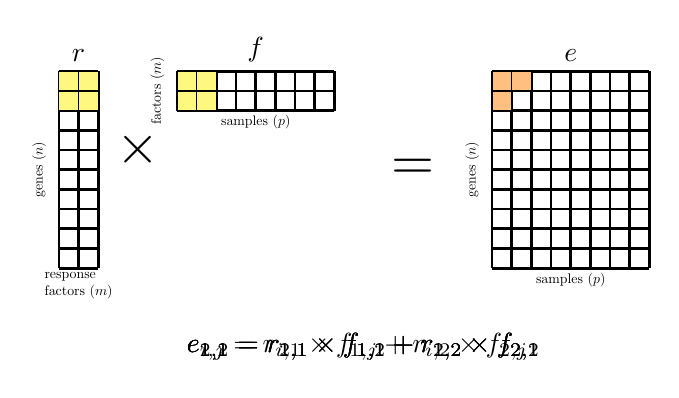
\begin{tikzpicture}[scale=0.5]
      %% \draw [help lines, opacity=0.5] (0,0) grid (22,12);
      %% \foreach \x in {1,2,...,19} \node [font=\small] at (\x,0) {\x};
      %% \foreach \y in {1,2,...,12} \node [font=\small] at (20,\y) {\y};

      \foreach \x in {0,0.5,1} \draw [-, line width=1] (\x,10) -- (\x,5);
      \foreach \y in {10, 9.5,...,5} \draw [-, line width=1] (0,\y) -- (1,\y);

      \foreach \x in {3,3.5,...,7} \draw [-, line width=1] (\x,10) -- (\x,9);
      \foreach \y in {10, 9.5, 9} \draw [-, line width=1] (3,\y) -- (7,\y);

      \node [rotate=90, scale=0.5] at (-0.5,7.5) {genes ($n$)};
      \node [below, align=left, scale=0.5] at (0.5,5) {response\\factors ($m$)};
      \node [below, scale=0.5] at (5,9) {samples ($p$)};
      \node [rotate=90, align=left, scale=0.5] at (2.5,9.5) {factors
        ($m$)};
      \node [scale=2] at (2,8) {$\times$};
      
      \node [above] at (0.5, 10) {$r$};
      \node [above] at (5,10) {$f$};

      \visible<2->{
        \node [scale=2] at (9,7.5) {$=$};
        \foreach \x in {11,11.5,...,15} \draw [-, line width=1] (\x,10) --
        (\x,5);
        \foreach \y in {10, 9.5,..., 5 } \draw [-, line width=1] (11,\y) --
        (15,\y);
        \node [below, scale=0.5] at (13,5) {samples ($p$)};
        \node [rotate=90, scale=0.5] at (10.5,7.5) {genes ($n$)};
        \node [above] at (13,10) {$e$};
      }

      \visible<3>{
        \draw [fill=yellow!50] (0,9.5) rectangle (0.5, 10);
        \draw [fill=yellow!50] (0.5,9.5) rectangle (1, 10);

        \draw [fill=yellow!50] (3,9.5) rectangle (3.5, 10);
        \draw [fill=yellow!50] (3,9) rectangle (3.5, 9.5);

        \draw [fill=orange!50] (11,9.5) rectangle (11.5, 10);
        \node [right] at (3,3) {$e_{1,1} = r_{1,1}\times f_{1,1} +
          r_{1,2}\times f_{2,1} $};
      }

      \visible<4>{
        \draw [fill=yellow!50] (0,9.5) rectangle (0.5, 10);
        \draw [fill=yellow!50] (0.5,9.5) rectangle (1, 10);

        \draw [fill=yellow!50] (3.5,9.5) rectangle (4, 10);
        \draw [fill=yellow!50] (3.5,9) rectangle (4, 9.5);

        \draw [fill=orange!50] (11.5,9.5) rectangle (12, 10);
        \node [right] at (3,3) {$e_{1,2} = r_{1,1}\times f_{1,2} +
          r_{1,2}\times f_{2,2} $};
      }

      \visible<5>{
        \draw [fill=yellow!50] (0,9) rectangle (0.5, 9.5);
        \draw [fill=yellow!50] (0.5,9) rectangle (1, 9.5);

        \draw [fill=yellow!50] (3,9.5) rectangle (3.5, 10);
        \draw [fill=yellow!50] (3,9) rectangle (3.5, 9.5);

        \draw [fill=orange!50] (11,9) rectangle (11.5, 9.5);
        \node [right] at (3,3) {$e_{2,1} = r_{2,1}\times f_{1,1} +
          r_{2,2}\times f_{2,1} $};
      }
      \visible<6>{
        \node [right] at (3,3) {$e_{i,j} = r_{i,1}\times f_{1,j} +
          r_{i,2}\times f_{2,j} $};
      }

%      \draw [-, line width=2,blue] (5,17) -- (18,17);

    \end{tikzpicture}
  \end{figure}
\end{frame}

\begin{frame}{matrix factorisation}
  \begin{figure}[ht]
    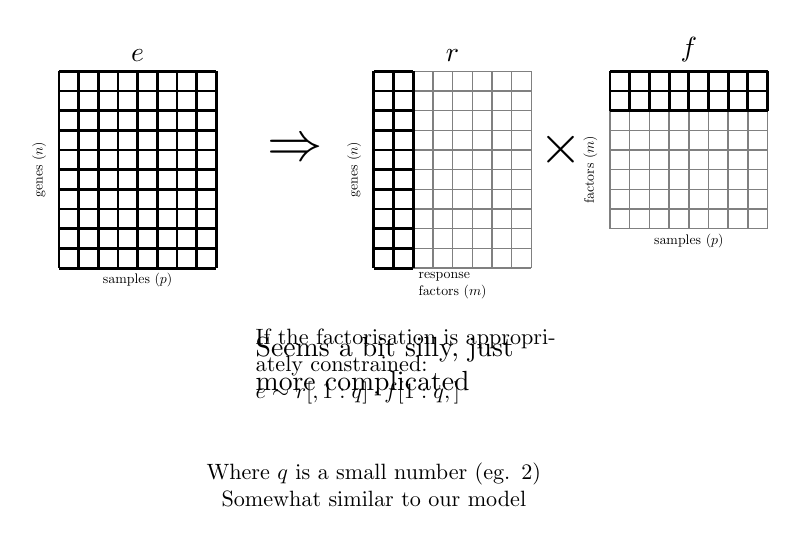
\begin{tikzpicture}[scale=0.5]
      %% \draw [help lines, opacity=0.5] (0,0) grid (22,12);
      %% \foreach \x in {1,2,...,19} \node [font=\small] at (\x,0) {\x};
      %% \foreach \y in {1,2,...,12} \node [font=\small] at (20,\y) {\y};

      \foreach \x in {0,0.5,...,4} \draw [-, line width=1] (\x,10) --
      (\x,5);
      \foreach \y in {10, 9.5,..., 5 } \draw [-, line width=1] (0,\y) --
      (4,\y);
      \node [below, scale=0.5] at (2,5) {samples ($p$)};
      \node [rotate=90, scale=0.5] at (-0.5,7.5) {genes ($n$)};
      \node [above] at (2,10) {$e$};
      
      \visible<2->{
      \foreach \x in {8,8.5,...,12} \draw [-, line width=0.5, gray] (\x,10) -- (\x,5);
      \foreach \y in {10, 9.5,...,5} \draw [-, line width=0.5, gray] (8,\y) -- (12,\y);

      \foreach \x in {14,14.5,...,18} \draw [-, line width=0.5, gray] (\x,10) -- (\x,6);
      \foreach \y in {10, 9.5,...,6} \draw [-, line width=0.5, gray] (14,\y) -- (18,\y);

      \node [rotate=90, scale=0.5] at (7.5,7.5) {genes ($n$)};
      \node [below, align=left, scale=0.5] at (10,5) {response\\factors ($m$)};
      \node [below, scale=0.5] at (16,6) {samples ($p$)};
      \node [rotate=90, align=left, scale=0.5] at (13.5,7.5) {factors
        ($m$)};
      \node [scale=2] at (6,8) {$\Rightarrow$};
      \node [scale=2] at (12.75,8) {$\times$};
      
      \node [above] at (10, 10) {$r$};
      \node [above] at (16,10) {$f$};
      }
      \visible<3>{
        \node [align=left, text width=4cm] at (9,2.5) {Seems a bit silly, just more complicated};
      }
      %% \visible<4>{
      %%   \node [align=left, text width=4cm, scale=0.8] at (9,2.5) {$e \sim r[,1:q] \cdot
      %%     f[1:q,]$ \\ \small where $q$ is a small number};      
      %% }
      \visible<4>{
        \node [align=left, text width=5cm, scale=0.8] at (9,2.5) {If the
          factorisation is appropriately constrained:\\$e \sim r[,1:q] \cdot
          f[1:q,]$};      
        \foreach \x in {8,8.5,9} \draw [-, line width=1] (\x,10) -- (\x,5);
        \foreach \y in {10, 9.5,...,5} \draw [-, line width=1] (8,\y) -- (9,\y);
        
        \foreach \x in {14,14.5,...,18} \draw [-, line width=1] (\x,10) -- (\x,9);
        \foreach \y in {10, 9.5,9} \draw [-, line width=1] (14,\y) -- (18,\y);

        \node [scale=0.8, align=center, text width=10cm] at (8,-0.5) {
          Where $q$ is a small number (eg. 2)\\
          Somewhat similar to our model};
      }
      
    \end{tikzpicture}
  \end{figure}
\end{frame}

\begin{frame}{matrix factorisation by \texttt{prcomp}}
  \begin{figure}[ht]
    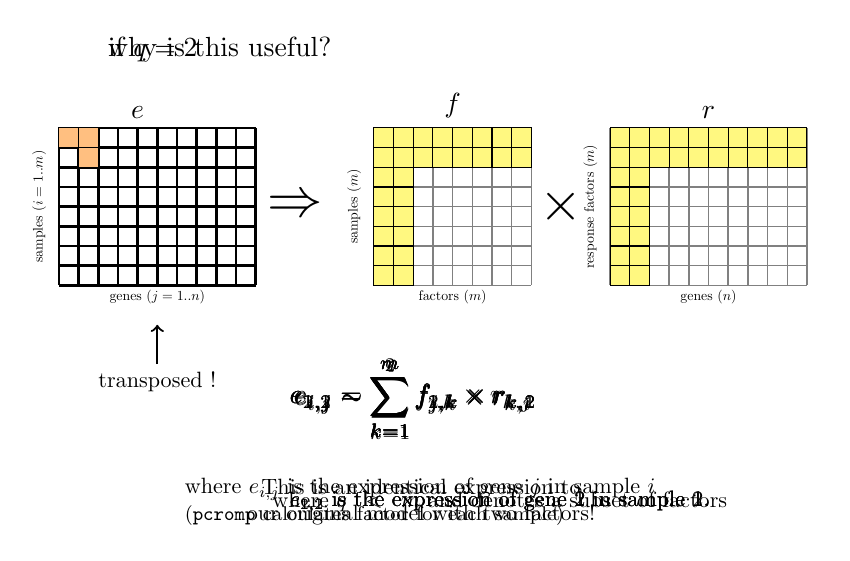
\begin{tikzpicture}[scale=0.5]
      %% \draw [help lines, opacity=0.5] (0,0) grid (22,12);
      %% \foreach \x in {1,2,...,19} \node [font=\small] at (\x,0) {\x};
      %% \foreach \y in {1,2,...,12} \node [font=\small] at (20,\y) {\y};

      \visible<2->{
        \foreach \x in {0,0.5,...,5} \draw [-, line width=1] (\x,10) --
        (\x,6);
        \foreach \y in {10, 9.5,...,6 } \draw [-, line width=1] (0,\y) --
        (5,\y);
        \node [below, scale=0.5] at (2.5,6) {genes ($j = 1..n$)};
        \node [rotate=90, scale=0.5] at (-0.5,8) {samples ($i = 1..m$)};
        \node [above] at (2,10) {$e$};
      }
      \visible<2>{
        \draw [->,thick] (2.5,4) -- (2.5,5);
        \node [below, scale=0.8] at (2.5,4) { transposed ! };
      }
      \visible<3->{
        \foreach \x in {8,8.5,...,12} \draw [-, line width=0.5, gray] (\x,10) -- (\x,6);
        \foreach \y in {10, 9.5,...,6} \draw [-, line width=0.5, gray] (8,\y) -- (12,\y);
        
        \foreach \x in {14,14.5,...,19} \draw [-, line width=0.5, gray] (\x,10) -- (\x,6);
        \foreach \y in {10, 9.5,...,6} \draw [-, line width=0.5, gray] (14,\y) -- (19,\y);
        
        \node [rotate=90, scale=0.5] at (7.5,8) {samples ($m$)};
        \node [below, align=left, scale=0.5] at (10,6) {factors ($m$)};
        \node [below, scale=0.5] at (16.5,6) {genes ($n$)};
        \node [rotate=90, align=left, scale=0.5] at (13.5,8) {response factors
          ($m$)};
        \node [scale=2] at (6,8) {$\Rightarrow$};
        \node [scale=2] at (12.75,8) {$\times$};
        
        \node [above] at (10, 10) {$f$};
        \node [above] at (16.5,10) {$r$};

      }
      \visible<3>{
        \node [align=left, text width=4cm] at (9,3.5) { $$ e_{i,j} = \sum_{k=1}^{m}{f_{i,k} \times r_{k,j}}   $$};

        \node [right, align=left, text width=8cm, scale=0.8] at (3,0.5) {
          where $e_{i,j}$ is the expression of gene $j$ in sample $i$\\
          \small(\texttt{pcromp} calculates factor for each sample) };
      }
      \visible<4>{
        \node [align=left, text width=4cm] at (9,3.5) { $$ e_{1,1} =
          \sum_{k=1}^{m}{f_{1,k} \times r_{k,1}}   $$};
        \draw [fill=orange!50] (0,9.5) rectangle (0.5,10);
        \foreach \x in {8,8.5,...,11.5} \draw [fill=yellow!50] (\x,9.5)
        rectangle (\x+0.5,10);
        \foreach \y in {9.5,9,...,6} \draw [fill=yellow!50] (14,\y) rectangle (14.5,\y+0.5);
        \node [right, scale=0.8, align=center, text width=10cm] at (3,0.5) {$e_{1,1}$ is the expression of gene 1 in sample 1.};
      }
      \visible<5>{
        \node [align=left, text width=4cm] at (9,3.5) { $$ e_{1,2} =
          \sum_{k=1}^{m}{f_{1,k} \times r_{k,2}}   $$};
        \draw [fill=orange!50] (0.5,9.5) rectangle (1,10);
        \foreach \x in {8,8.5,...,11.5} \draw [fill=yellow!50] (\x,9.5)
        rectangle (\x+0.5,10);
        \foreach \y in {9.5,9,...,6} \draw [fill=yellow!50] (14.5,\y) rectangle (15,\y+0.5);
        \node [right, scale=0.8, align=center, text width=10cm] at (3,0.5) {
          $e_{1,2}$ is the expression of gene 2 in sample 1.};
      }
      \visible<6>{
        \node [align=left, text width=4cm] at (9,3.5) { $$ e_{2,2} =
          \sum_{k=1}^{m}{f_{2,k} \times r_{k,2}}   $$};
        \draw [fill=orange!50] (0.5,9) rectangle (1,9.5);
        \foreach \x in {8,8.5,...,11.5} \draw [fill=yellow!50] (\x,9)
        rectangle (\x+0.5,9.5);
        \foreach \y in {9.5,9,...,6} \draw [fill=yellow!50] (14.5,\y) rectangle (15,\y+0.5);
        \node [right, scale=0.8, align=center, text width=10cm] at (3,0.5) {
          $e_{2,2}$ is the expression of gene 2 in sample 2.};
      }
      
      \visible<7>{
        \node [right,align=left, text width=8cm, align=left] at (1,12) {why is this
          useful?};
        \node [align=left, text width=4cm] at (9,3.5) { $$ e_{i,j} \sim
          \sum_{k=1}^{q}{f_{j,k} \times r_{k,i}}   $$};
        \node [right, scale=0.8, align=center, text width=10cm] at (3,0.5) {
          where $q < m$ and denotes a subset of factors};
        
      }
      \visible<8>{
        \foreach \y in {9.5,9.0,...,6} \draw [fill=yellow!50] (8,\y) rectangle (8.5,\y+0.5);
        \foreach \y in {9.5,9.0,...,6} \draw [fill=yellow!50] (8.5,\y) rectangle (9,\y+0.5);

        \foreach \x in {14,14.5,...,18.5} \draw [fill=yellow!50] (\x,9.5) rectangle (\x+0.5,10);
        \foreach \x in {14,14.5,...,18.5} \draw [fill=yellow!50] (\x,9) rectangle (\x+0.5,9.5);
       
        \node [align=left, text width=4cm] at (9,3.5) { $$ e_{i,j} \sim
          \sum_{k=1}^{2}{f_{j,k} \times r_{k,i}}   $$};
        \node [right,align=left, text width=8cm, align=left] at (1,12) {if $q
          = 2$};       
        \node [right, scale=0.8, align=center, text width=10cm] at (1,0.5) {
          This is an identical expression to our original model with two factors!};
      }

    \end{tikzpicture}
  \end{figure}
\end{frame}

\begin{frame}{the factors and the metadata}
  \begin{figure}[ht]
    \begin{tikzpicture}[scale=0.5]
      %% \draw [help lines, opacity=0.5] (0,0) grid (22,12);
      %% \foreach \x in {1,2,...,19} \node [font=\small] at (\x,0) {\x};
      %% \foreach \y in {1,2,...,12} \node [font=\small] at (20,\y) {\y};
      \visible<1->{
        \foreach \x in {0,0.5,...,4} \draw [-, line width=0.5, gray] (\x,10) -- (\x,6);
        \foreach \y in {10, 9.5,...,6} \draw [-, line width=0.5, gray] (0,\y) -- (4,\y);
        
%        \foreach \x in {14,14.5,...,19} \draw [-, line width=0.5, gray] (\x,10) -- (\x,6);
%        \foreach \y in {10, 9.5,...,6} \draw [-, line width=0.5, gray] (14,\y) -- (19,\y);
        
         \node [rotate=90, scale=0.5] at (-0.5,8) {samples ($m$)};
         \node [below, align=left, scale=0.5] at (2,6) {factors ($m$)};
        %% \node [below, scale=0.5] at (16.5,6) {genes ($n$)};
        %% \node [rotate=90, align=left, scale=0.5] at (13.5,8) {response factors
        %%   ($m$)};
        %% \node [scale=2] at (6,8) {$\Rightarrow$};
        %% \node [scale=2] at (12.75,8) {$\times$};
        
        \node [above] at (2, 10) {$f$};
        %% \node [above] at (16.5,10) {$r$};

      }

      
      \visible<2->{
        \node [scale=2] at (6,8) {$\Rightarrow$};
        \node [below right] at (9,13) {\begin{tikzpicture}[scale=0.35]
            \node [right, rotate=90, scale=0.8] at (7,8) {Tissue};
            \node [right, rotate=90, scale=0.8] at (8,8) {Age};
            \node [right, rotate=90, scale=0.8] at (9,8) {Condition};
            \node [right, rotate=90, navy, scale=0.8] at (10,8) {RNA conc.};
            \node [right, rotate=90, navy, scale=0.8] at (11,8) {date};
            \node [right, rotate=90, navy, scale=0.8] at (12,8) {user};
            \node [right, rotate=90, navy, scale=0.8] at (13,8) {cDNA yield};
            \node [right, rotate=90, navy, scale=0.8] at (14,8) {RNA cond.};
            \node [right, rotate=90, navy, scale=0.8] at (15,8) {method};
            
            \draw [-] (6,8) -- (16.5,8);
            \draw [-] (6.5,10) -- (6.5,0);
            \node [above, rotate=90, scale=0.8] at (6.3,5) {samples};
            \foreach \x in {7.5, 8.5, ..., 17.5} \draw [-,dotted, opacity=0.5] (\x,10) -- (\x,0);
            \foreach \y in {7.5, 7, ..., 0} \draw [-,dotted, opacity=0.5] (6,\y)
            -- (18.5,\y);
            \end{tikzpicture}
          };
      }
    \end{tikzpicture}
  \end{figure}
  
\end{frame}

\begin{frame}[fragile]{prcomp}
  \begin{columns}
    \begin{column}{0.5\textwidth}
      \begin{rcode}
## exp.data is a data set of 15,923 genes (rows)
## and 54 samples (columns)
> pca.l1 <- prcomp( t(log(exp.data)), 
     scale=TRUE )
> names(pca.l1)
[1] "sdev" "rotation" "center" "scale" "x"
> dim(pca.l1$x)
[1] 54 54
> dim(pca.l1$rotation)
[1] 15923    54
      \end{rcode}
    \end{column}

    \begin{column}{0.5\textwidth}
      \small
      \begin{itemize}
      \item \textcolor{navy}{x} is equivalent to $f$, the matrix of factor levels
      \item \textcolor{navy}{rotation} is equivalent to $r$ (the matrix of factor response
        rates) transposed.
      \end{itemize}
    \end{column}
  \end{columns}

  \begin{figure}[ht]
    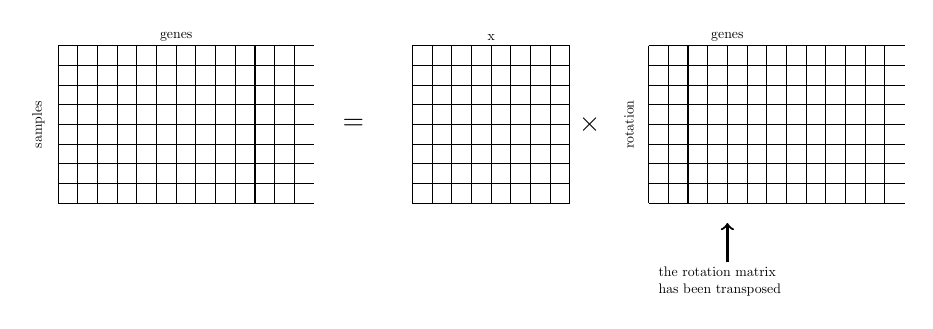
\begin{tikzpicture}[scale=0.5]
      %% \draw [help lines, opacity=0.5] (0,0) grid (22,12);
      %% \foreach \x in {1,2,...,19} \node [scale=0.5] at (\x,0) {\x};
      %% \foreach \y in {1,2,...,12} \node [scale=0.5] at (20,\y) {\y};
      
      \node [above, scale=0.5] at (3,10) {genes};
      \foreach \x in {0,0.5,...,6} \draw [-] (\x,10) -- (\x,6);
      \node [scale=0.5, rotate=90] at (-0.5,8) {samples};
      \foreach \y in {10,9.5,...,6} \draw [-] (0,\y) -- (6.5,\y);


      \node [scale=1] at (7.5, 8) {$=$};
      
      \node [above, scale=0.5] at (11,10) {x};
      \foreach \x in {9,9.5,...,13} \draw [-] (\x,10) -- (\x,6);
      \foreach \y in {10,9.5,...,6} \draw [-] (9,\y) -- (13,\y);

      \node [scale=1] at (13.5,8) {$\times $};

      \node [above, scale=0.5] at (17,10) {genes};
      \node [scale=0.5,rotate=90] at (14.5,8) {rotation};
      \foreach \x in {15,15.5,...,21} \draw [-] (\x,10) -- (\x,6);
      \foreach \y in {10,9.5,...,6} \draw [-] (15,\y) -- (21.5,\y);

      \draw [->, thick] (17,4.5) -- (17,5.5);
      \node [scale=0.5, below, text width=3.5cm, align=left] at (17,4.5)
      {the rotation matrix has been transposed};

   \end{tikzpicture}
  \end{figure}
\end{frame}

\begin{frame}[fragile]{reversing the PCA}
  \begin{rcode}
    > pc.rev <- pca.l1$x %*% t(pca.l1$rotation)
    > par(mfrow=c(1,2))
    > plot( pc.rev[,1], log(exp.data)[1,] )
    > plot( pca.l1$center[1] + pc.rev[,1] * pca.l1$scale[1], 
           log(exp.data)[1,] )
  \end{rcode}
  
  \begin{figure}[ht]
    \includegraphics[width=\textwidth]{data/pca_gene1_recovered.pdf}
  \end{figure}
\end{frame}

\begin{frame}[fragile]{completing the reversion}
  \begin{rcode}
    pc.rev <- pca.l1$x %*% t(pca.l1$rotation) 
    pc.rev <- t(pc.rev)   ## transpose
    ## then recover the scale
    pc.rev <- pc.rev * pca.l1$scale
    pc.rev <- pc.rev + pca.l1$center
    ## reverse the log transformation
    pc.rev <- exp(pc.rev)
    ## plot a subset of the genes 
    plot(exp.data[1:100,], pc.rev[1:100,],
    abline(0,1, col='red')
  \end{rcode}
  \begin{figure}[ht]
    \includegraphics[width=0.5\textwidth]{data/pca_recovered.pdf}
  \end{figure}
\end{frame}

\begin{frame}[fragile]{partial reversions}
  \begin{rcode}
 partial.rev <- lapply(1:54, function(i){
   r <- t(pca.l1$x[,1:i, drop=FALSE] %*% t(pca.l1$rotation[,1:i,drop=FALSE]))
   r})
 
 par(mfrow=c(2,3))
 for(i in 1:6){
   plot( partial.rev[[i]][1:100,], t(scale(t(log(exp.data[1:100,])))),
   main=paste(``dims'', 1, ``to'', i), xlab='recovered', ylab='real')
   e <- sum( (partial.rev[[i]] - t(scale(t(log(exp.data)))))^2 )
   legend('topleft', legend=paste('SS:', sprintf('%.2e', e)), bty='n', cex=2)
 }
 \end{rcode}
 \vspace{-0.5cm}
  \begin{figure}[ht]
    \includegraphics[width=0.8\textwidth]{data/partial_recoveries}
  \end{figure}
\end{frame}

\begin{frame}[fragile]{Sum of Squared deviates}
  \begin{rcode}
    ss.dim <- sapply( partial.rev, function(x){
         sum( ( x - t(scale(t(log(exp.data)))) )^2 )})

    pdf("sqSum_dims.pdf", width=5, height=5)
    plot( ss.dim, xlab='dimensions used', ylab='sum of squared errors' )
    abline(h=0, col='red')
    dev.off()
  \end{rcode}
  
  \begin{figure}[ht]
    \includegraphics[width=0.4\textwidth]{data/sqSum_dims}
  \end{figure}
\end{frame}

\begin{frame}[fragile]{Why didn't I unscale the data?}
  \begin{rcode}
  ss.dim <- sapply( partial.rev, function(x){
    sum( ( x - t(scale(t(log(exp.data)))) )^2 )})
  
  pdf("sqSum_dims.pdf", width=5, height=5)
  plot( ss.dim, xlab='dimensions used', ylab='sum of squared errors' )
  abline(h=0, col='red')
  dev.off()
  \end{rcode}
  \pause
  \vspace{-0.5cm}
  \begin{figure}[ht]
    \includegraphics[width=0.9\textwidth]{data/recoverd_scaled.pdf}
  \end{figure}
\end{frame}

\begin{frame}[fragile]{Why so good?}
  The majority of the information is in the:

  \textcolor{navy}{\texttt{pca.l1\$center} }
  
  Which represents the basal expression level $b$ in:

  $$
    E_j = b + r_1\times f_{1,j} + r_2\times f_{2,j}
  $$
  
    The other terms have much smaller effects.

\end{frame}

\begin{frame}{Interesting features}
  
  {\small
  Define a score that relates to differential expression between
  classes.

  For two class problems, one can use the t-statistic, for more than two
  classes the f-statistic can be used.

  The t-statistic can be considered as:
  
  $$ \frac{difference\, between\, means}{standard\, deviation} $$

  The f-statistic is simply:
  
  $$ \frac{variance\, between\, class\, means}{variance\, within\, classes} $$

  This can easily be obtained in R using the \texttt{lm} function which also allows
  you to specify much more elaborate linear models. But it can be a bit slow, and
  for a quick check using a one-way Anova, I prefer my own custom function:
}
\end{frame}

\begin{frame}[fragile]{a vectorised f-stat}
  The data should be in a matrix called d, with samples in columns and
  features in rows. Each sample should belong to a class which is specified
  in a numeric vector called \texttt{d.g}.

  \begin{rcode}
    g.ids <- sort(unique(d.g))
    g.sizes <- vector(mode='numeric', length=length(g.ids))
    g.means <- matrix(nrow=nrow(d), ncol=length(g.ids))
    means <- rowSums( d ) / ncol( d ) ## faster than rowMeans, but not as safe
    var.within <- rep(0, nrow(d))
    var.between <- var.within
    N <- ncol( d )        ## the number of samples
    K <- length( g.ids )  ## the number of groups
    for(i in 1:length(g.ids)){
      c.i <- which(d.g == g.ids[i])
      g.sizes[i] <- length(c.i)
      g.means[,i] <- rowSums(d[ ,c.i, drop=FALSE]) / g.sizes[i]
      ## we also need the internal variances, but the way we combine these
      ## means that we can't just cal var if I recall correctly.
      var.within <- var.within + ( rowSums((d[,c.i, drop=FALSE] - g.means[,i])^2) / (N - K) )
      var.between <- var.between + ( g.sizes[i] * ((g.means[,i] - means)^2) / (K - 1) )
    }
    f <- var.between / var.within
  \end{rcode}
\end{frame}

\begin{frame}[fragile]{get some fstats}
  
  {\footnotesize
  To get a vector containing a numerical representation of the sample classes of each column
  I use a function defined in \texttt{general\_functions.R}.
  \begin{rcode}
    source("~/R/general_functions.R")
    sample.mf <- mulFactor(samples, c('genotype', 'tissue', 'drug'))
  \end{rcode}

  Then I use the \texttt{fStats} function defined in the same file. This returns a named list
  containing the f statistic itself and the degrees of freedom associated with the test (which
  allows me to use \texttt{pf} to get probabilities associated with the f-statistics).
  \begin{rcode}
    ## and then we can get some fstats, to see what pops up..
    fstats.a <- fStats(log(exp.data), sample.mf$f)
    
    ## we can use order to provide an index of the original data ordered
    ## by the f statistic
    fstat.a.o <- order(fstats.a$f, decreasing=TRUE)
  \end{rcode}

  For plotting purposes it's nice to order the samples in a reasonable manner:
  \begin{rcode}
    ## lets make a reasonable sample order...
    sample.o <- order(samples[,'tissue'], samples[,'genotype'], samples[,'drug'])
    samples[sample.o,]
    ## ahah, now I understand the experimental design...
  \end{rcode}

  we can now write a plot function and look at some individual plots:
}
\end{frame}

\begin{frame}[fragile]{a plot function}
  \begin{rcode}
    ## this function makes use of global variables. These can't be modified,
    ## but can still result in unexpected behaviour
    plotExp <- function(ind, interactive=TRUE){
      for(j in ind){
        mx <- max(exp.data[j,])
        mn <- min(exp.data[j,])
        plot(1:length(sample.o), exp.data[j, sample.o],
             type='n', col=as.factor(samples[sample.o,'drug']), pch=19,
             ylim=c( mn - (mx-mn)*0.05, mx ),
             main=paste(feat.data[j,'Gene symbol']), ylab='Expression', xlab='Sample')
        usr <- par("usr")
        ## set up some rectangles to indicate the tissue type.
        rect((1:length(sample.o))-0.5, usr[3], (1:length(sample.o))+0.5, usr[4],
             col=hsvScale(as.numeric(as.factor(samples[sample.o,'tissue'])), 
                          sat=0.5, alpha=0.5), border=NA)
        ## and to indicate the genotype
        rect((1:length(sample.o))-0.5, usr[3], (1:length(sample.o))+0.5, usr[3] + (mx-mn)*0.05,
             col=hsvScale(as.numeric(as.factor(samples[sample.o,'genotype'])), 
             sat=c(0.5), alpha=0.6), border=NA)
        
        points(1:length(sample.o), exp.data[j, sample.o], type='b',
        pch=19, col=as.factor(samples[sample.o,'drug']) )
        if(interactive)
            inp <- readline(paste(feat.data[j,'Gene symbol'], ":"))
      }
    }
  \end{rcode}
\end{frame}

\begin{frame}[fragile]{Some plots}
  \begin{figure}[ht]
    \includegraphics[width=0.7\textwidth]{images/fstatAll}
  \end{figure}
  \vspace{-3ex}
  \begin{rcode}
    par(mfrow=c(3,3)
    plotExp(fstat.a.o[1:9])
  \end{rcode}
\end{frame}

\begin{frame}[fragile]{Look for drug effect in liver}
  \begin{rcode}
    liver.b <- samples[,'tissue'] == 'liver'

    fstats.dl <- fStats(log(exp.data[,liver.b]), as.numeric(as.factor(samples[liver.b,'drug'])))
    fstats.dl.o <- order(fstats.dl$f, decreasing=TRUE)
    ## again, the fstats are kept in the fstats.dl$f vector
    par(mfrow=c(3,4))
    plotExp(fstats.dl.o[1:12])
  \end{rcode}
  
\end{frame}

\begin{frame}{Plots}
  \begin{figure}[ht]
    \includegraphics[width=\textwidth]{images/fstatsDrugLiver}
  \end{figure}
\end{frame}

\begin{frame}{What do we see?}
  \begin{itemize}
  \item Big seperation of tissues.\\
    If we didn't see this the data would be useless though.
  \item Some effect of drugs.
  \item Drug effect generally away from the normal (lean).\\
    That is the drug doesn't seem to work.
  \item We may need to look at effects of drug on genes that
    are affected by the fatty phenotype.\\
    $\Rightarrow$ refine statistical questions.
  \end{itemize}
  
  We can get an overview of the data pretty easily, but to answer specific
  questions we have to specify those in statistical terms. This relates
  directly to the biology.
\end{frame}

%% \begin{frame}{next?}
%% We'll have a look at this data set together on Friday.

%% Please bring your laptops. With R!
%% \end{frame}

\end{document}
